%\documentclass{article}
\documentclass{chi2009}
\usepackage{times}
%\usepackage{uist}
\usepackage{url}
\usepackage{graphics}
\usepackage{color}

% \newcommand{\want}[1]{{[\color{blue} WANT: #1]}}
% \newcommand{\todo}[1]{{[\color{blue} TODO: #1]}}
% \newcommand{\idea}[1]{{[\color{blue} IDEA: #1]}}
% \newcommand{\node}[1]{{[\color{blue} NOTE: #1]}}

\newcommand{\want}[1]{}
\newcommand{\todo}[1]{}
\newcommand{\idea}[1]{}
\newcommand{\node}[1]{}




\begin{document}

% --- Copyright notice ---
\conferenceinfo{UIST'09}{October 4-7, 2008, Victoria, BC, Canada}
\CopyrightYear{2009}
\crdata{x-xxxxx-xxx-x/xx/xxxx}

% Uncomment the following line to hide the copyright notice
\toappear{}
% ------------------------

\bibliographystyle{plain}

\title{Exposing Disputed Statements on the Web}

%%
%% Note on formatting authors at different institutions, as shown below:
%% Change width arg (currently 7cm) to parbox commands as needed to
%% accommodate widest lines, taking care not to overflow the 17.8cm line width.
%% Add or delete parboxes for additional authors at different institutions. 
%% If additional authors won't fit in one row, you can add a "\\"  at the
%% end of a parbox's closing "}" to have the next parbox start a new row.
%% Be sure NOT to put any blank lines between parbox commands!
%%

\author{
\parbox[t]{9cm}{\centering
	     {\em Author names removed for blind review}\\
}
}

\maketitle

%RULE: Don't cite media reports unless I have to

\abstract
Think Link is a tool that helps a user know when information they read on a web page is disputed. As a user browses the web, Think Link highlights snippets of text that make claims that conflict with information on other web sites. If a user clicks on a highlighted snippet then Think Link will show them an argument graph showing the best evidence for and against the claim being true.

All information in Think Link is provided by users. Think Link is designed to support two usage scenarios: (i) Activists care strongly about a particular issue and combine Think Link with a search engine to find and mark places where web sites say things that they disagree with; and (ii) Sceptical Readers install Think Link as a browser extension so that they can see when things they read are disputed and find other sources that present an alternative viewpoint.

\classification{H5.2 [Information interfaces and presentation]:
User Interfaces. - Graphical user interfaces.}

\terms{Design, Human Factors}

\keywords{Sensemaking, Annotation, Argumentation, Web, CSCW}


\tolerance=400 
  % makes some lines with lots of white space, but 	
  % tends to prevent words from sticking out in the margin

\section{INTRODUCTION}

The web contains a huge amount of information, but not all of this information is accurate~\cite{Mintz2002,Neumann2003,Resnik1998,Zhou2004} and some web sites present only one side of a contentious issue~\cite{Herman2002,Gentzkow2007}. If a user is to gain a broad understanding of a topic then they will need to either stick to sources that they trust to provide accurate and balanced information or spend time looking for information on other web sites that conflicts with what they have read. Even if a user tries hard to research every topic they read, they can still get caught out by claims that they had not realized were disputed.
\todo{word this better}\todo{update all screenshots}

In this paper we present Think Link, a tool that helps users discover when information they read conflicts with information on other web sites, and helps users find alternative sources that provide different points of view. When Think Link is used as a browser plugin it will highlight text that makes a disputed claim (Figure~\ref{highlight}). When a user clicks on a highlighted snippet, Think Link presents them with an argument graph that shows the best evidence for and against the claim, as voted for by other Think Link users (Figure~\ref{claimview}). 

\begin{figure}[tb]
	\begin{center}
	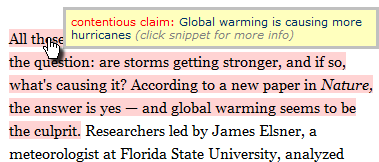
\includegraphics[width=5cm]{../screenshots/highlight_crop.png}
	\caption{Think Link highlights snippets that make disputed claims}
	\label{highlight}
	\end{center}
\end{figure}

Think Link relies on users to identify disputed claims, to find instances of these claims on web sites, and to vote for which sources provide the best support or opposition for a claim. 
Think Link is designed to cater to two groups of people:

\begin{description}
\item[Activists] care strongly about particular issues. They use Think Link to find and mark instances of claims that this disagree with so that other readers will see that these claims are disputed and be exposed to the opposing point of view.

\item[Sceptical Readers] want to know when information they read is disputed. They install Think Link as a browser plugin so that it will highlight disputed claims and show them the best evidence supporting opposing points of view.
\end{description}

\begin{figure}[tb]
	\begin{center}
	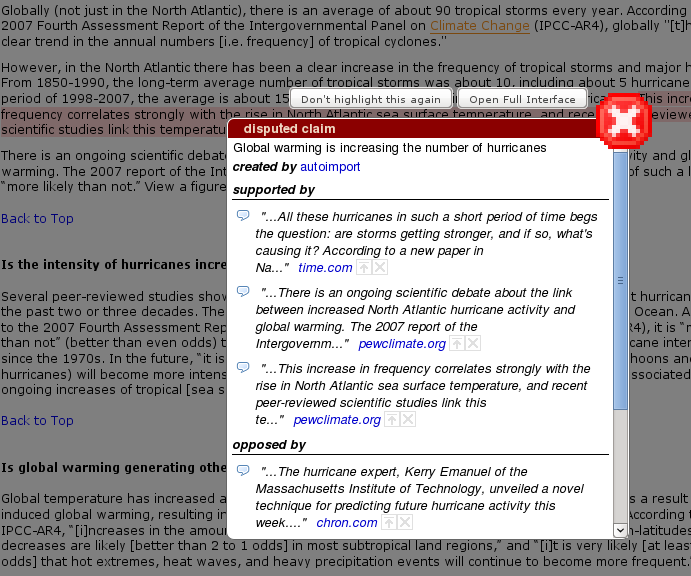
\includegraphics[width=5cm]{../screenshots/v2_popup_dim.png}
	\caption{Click on a claim to investigate evidence for and against it}
	\label{claimview}
	\end{center}
\end{figure}

\todo{Claim panel should have 'more' buttons}


The design of Think Link was guided by two user studies, in which we observed the behavior of users as they perfomed tasks fitting the usage scenarios for Activist and Sceptical Reader.

\todo{Talk about automatically including all arguments from Snopes}
\todo{I think we need to do some kind of evaluation of the new interface, even if it is just showing it to some people, or having people in the lab try it.}
\todo{Need figures saying how efficient it is for an activist user to mark up a topic}

% \begin{figure}[tb]
% 	\begin{center}
% 	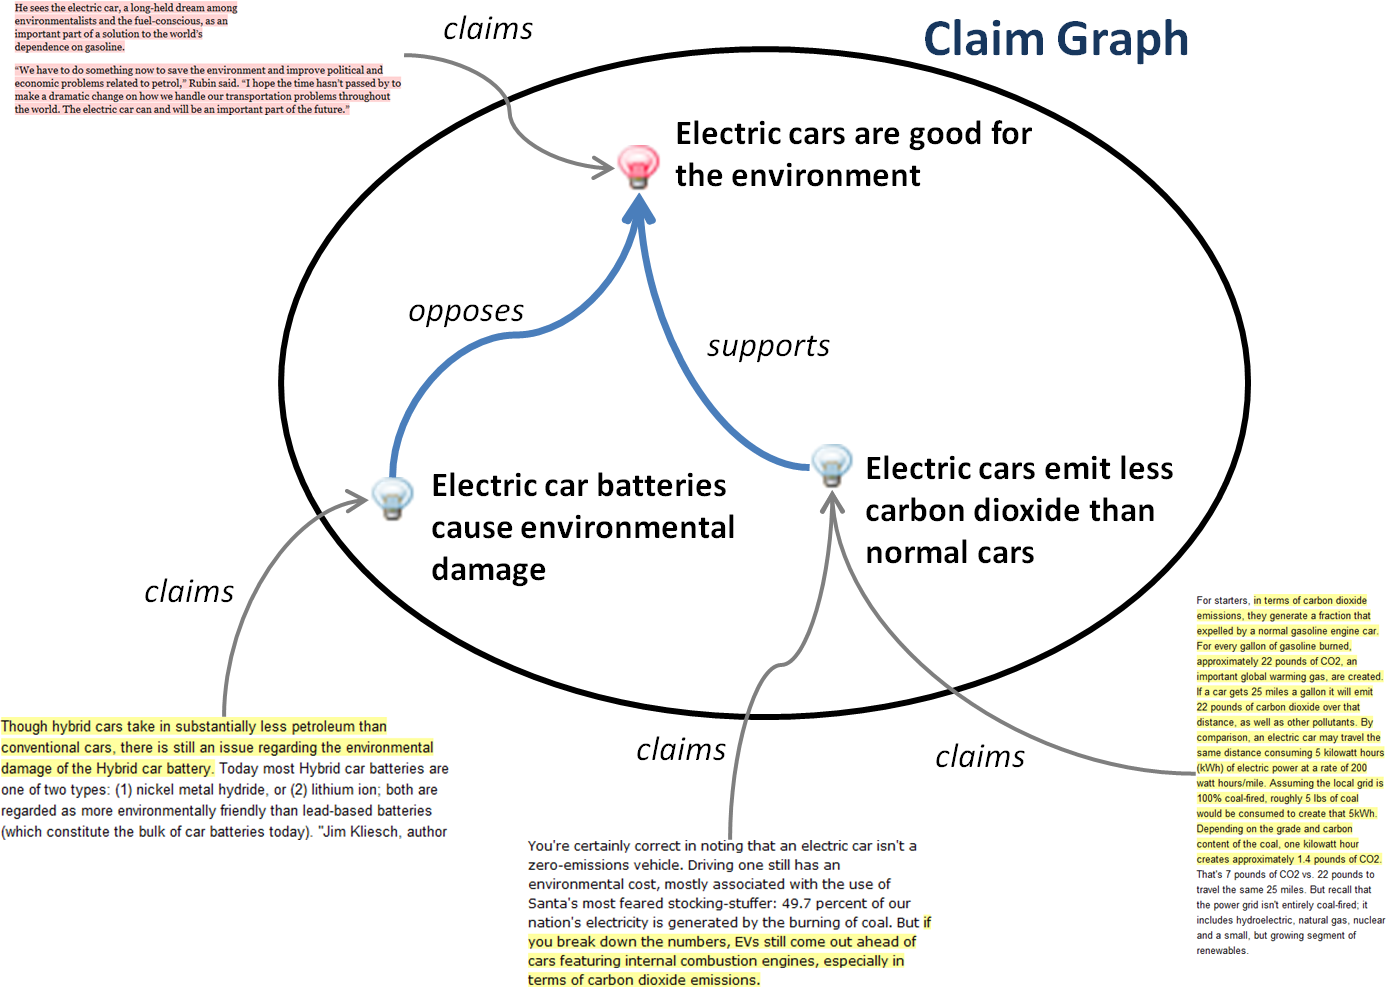
\includegraphics[width=7.7cm]{../screenshots/summary_graph.png}
% 	\caption{Think link connects claims to each other and to web snippets}
% 	\label{summarygraph}
% 	\end{center}
% \end{figure}


\section{Related Work}
\todo{Don't cite things that aren't relevant}

Think Link builds on work in several different areas. The argumentation structure influenced by IBIS~\cite{Rittel1973} tools such as gIBIS~\cite{Conklin1987a}. The idea of highlighting information that may not be trustworthy was previously applied to Wikipedia by WikiTrust~\cite{Adler2008a}. The model of using a community to collect and filter information from a range of sources is influenced by tagging systems~\cite{Marlow2006}. The idea of gathering up a collection of snippets from web pages has been used by clipping tools such as Internet Scrapbook~\cite{Sugiura1998}. 

What makes Think Link interesting is the way that it combines ideas from these different domains and applies them to the task of showing users when the information they read conflicts with information from other sources.

\subsection{Argumentation and Design Rationale}

Think Link's argument graph is inspired by Issue Based Information System (IBIS)~\cite{Rittel1973} tools such as gIBIS~\cite{Conklin1987a}, Compendium~\cite{Selvin2001}, Collabatorium~\cite{Klein2007}, Zeno~\cite{Gordon1997}, and Cohere~\cite{Shum2008} model arguments as a graph of connected ideas. While the graph structure varies between tools, most tools allow one to mark a claim as supporting or opposing another claim, and allow one to mark an claim as relating to an issue. 

Although Think Link's argument graph is very similar to that used by IBIS tools, it uses it for a different purpose. In Think Link the focus is on the snippets, and the purpose of the argument graph is to organize snippets, identify when snippets are disputed, and identify which snippets provide the best evidence for a particular point of view. A user is encouraged to create a new claim only when they want to group together a large number of snippets that make that claim, and a user is expected to form an opinion primarily by looking at the snippets that make that claim, rather than by looking at the argument graph itself. This differs from the normal way in which previous IBIS tools have been used. In a tool such as gIBIS~\cite{Conklin1987a} the focus is on the argument graph. A user is encouraged to break their argument down into as many separate ideas as possible and a user is expected to use the graph itself to reach a conclusion. In Think Link it is perfectly acceptable to have a claim that is not linked to any other claims or topics, but is associated with many topics --- this would not fit with the expected usage model for other IBIS tools.

Isenmann and Reuter~\cite{Isenmann1997} identify a number of problems with using IBIS tools to help people resolve disputes and make decisions. Broadly speaking, they found that opposing groups were unkeen to agree to use an IBIS tool to resolve their dispute, and that users found it difficult to properly encode a complex issue as an argument graph. We believe that while the problems they observe are important when an IBIS tool is being used for conflict modelling and resolution they are less of a problem for a tool like Think Link that is designed primarily for conflict discovery.

Cohere~\cite{Shum2008} allows a user to associate a web page with a claim in an argument graph and provides a Firefox plugin to help users do this; however Cohere and Think Link have very different models. In Cohere, when one creates a new claim one can specify one or more URLs to be used as supporting evidence. Cohere is not intended to be used as a tool to identify disputed snippets, and does not expect users to attach large numbers of web snippets to existing claims.

Think Link uses a simple IBIS-like graph structure in which claims support, oppose, or relate-to other claims. Several alternative graph structures have been proposed for describing arguments and design rationale. WinWin~\cite{Boehm2006} models the different stakeholders and their different motives. The Toulmin Model~\cite{toulmin1958} breaks down the logical way in which arguments are formed from evidence, rules, and exceptions. QOS~\cite{Maclean1991} explicitly states the criteria used to choose between positions. More formal models such as Carneades~\cite{Gordon2007} have been used for artificial intelligence.

Think Link's argument visualization is influenced by the left-to-right layout of Cohere~\cite{Shum2008}. Compendium~\cite{Selvin2001} contains a number of other visualizations of argument graphs. Mess Maps~\cite{Horn2007} present an alternative view in which an argument is divided into different sectors, each of which presents the argument from a different frame of discourse (e.g. policy maker vs industrialist vs environmentalist).



\subsection{Checking Accuracy and Bias on the Web}

If one sees a claim on the web that one suspects might be untrue then one can look it up on Snopes\footnote{http://snopes.com} or FactCheck\footnote{http://factcheck.org}. Snopes is a database of urban legends that the site owners have investigated to determine whether they are true or not. FactCheck is a web site that investigates claims being made by US political parties and attempts to uncover the facts. Think Link's database automatically imports all contentious claims identified by Snopes. FactCheck updates infrequently enough that we have been able to manually add its disputed claims to Think Link as they appear.

NewsCube~\cite{Park2009} and MediaCloud\footnote{http://mediacloud.org} use statistics to help readers avoid media bias. NewsCube presents a user with articles on the same topic that have different biases. MediaCloud applies various statistical analyses to news sources so that a reader can see when different news sources associate different words with the same topic.

Several authors have investigated ways to make Wikipedia\footnote{http://wikipedia.org} more trustworthy. WikiTrust~\cite{Adler2008a} highlights passages on wikipedia based on the likelihood that another user will change that text in the future --- recent edits by untrusted editors are marked as less trustworthy than old edits by trusted editors. Wiki Dashboard~\cite{Kittur2008} presents the reader of a Wikipedia article with a visualization that shows them how it has been edited in the past and lets them see graphically how contentious the topic is. Wiki Scanner\footnote{http://wikiscanner.virgil.gr} finds Wikipedia edits that have been made by people with an interest in spreading misinformation (e.g. people from a company editing pages about that company).

% 
% 
% NewsCube~\cite{Park2009}.
% Wikipedia fixes Vandalism~\cite{Viegas2004}.
% Trustworthiness~\cite{Gil2006}.
% WikiTrust~\cite{Adler2008}. Wiki Dashboard~\cite{Kittur2008}.
% Wiki Scanner\footnote{http://wikiscanner.virgil.gr}.
% SourceWatch\footnote{http://sourcewatch.org}, Snopes\footnote{http://snopes.com}, FactCheck\footnote{http://factcheck.org}.

\subsection{Annotating, Tagging, Clipping, and Open Hypermedia}

Think Link is an example of an Open Hypermedia system~\cite{Bouvin2000}. Like other Open Hypermedia systems, Think Link allows users to lay an additional link structure over an existing hypertext document. Think Link differs from prior open hypermedia systems in its focus on revealing contentious arguments. While other systems such as HyperDISCO~\cite{Wiil1996} could be used to link a snippet to a contentious claim, they do not provide user interface support to make this easy.

\todo{Say how different from other Open Hypermedia link annotation systems}

Tagging Systems~\cite{Marlow2006,Golder2006} allow users to collect and organize information by associating it with an ad-hoc collection of tags. Notable tagging systems include del.icio.us\footnote{http://del.icio.us} which uses tags to organize web pages, and Flickr\footnote{http://flickr.com} which associates tags with photos. 

Annotation tools~\cite{Marshall1998} such as Annotea~\cite{Koivunen2001} and ScreenCrayons~\cite{Olsen2004} allow users to highlight sections of text on a page. Annotation systems often also do clipping. Clipping tools such as Internet Scrapbook~\cite{Sugiura1998}, Hunter Gatherer~\cite{Schraefel2002}, ScratchPad~\cite{Gotz2007}, ClipMarks\footnote{http://clipmarks.com}, and Diigo\footnote{http://diigo.com} allow users to collect text snippets from web pages, tag them, and share them with friends. In some cases, other users who see a web page an see text highlighted where other users have clipped it. These tools do not attempt to identify when snippets make disputed claims or to connect them to opposing sides of an argument.

ClaimSpotter~\cite{Sereno2005,Sereno2004} allows one to mark up a scholarly paper with logical triples (subject, verb, object) describing interesting claims that are being made in the document. This semantic information can be used to connect claims in different documents. Entity Workspace~\cite{Bier2006} does something similar for intelligence documents. Unlike Think Link, these tools are looking for logical relations between entities rather than instances of already-known claims.

SpinSpotter\footnote{http://spinspotter.com} allows a user to highlight snippets of text that contain spin or bias and either describe why the text is biased, or rewrite the text in an unbiased way. While SpinSpotter and Think Link share a goal of drawing user attention to biased or inaccurate information, they do so in a different way. SpinSpotter annotates a snippet with an annotation specific to that particular snippet of text, while Think Link treats a snippet as being an instance of a shared contentious claim, and links all snippets identified as making that claim to a shared graph node linking to other information about that claim.

Videolyzer~\cite{Diakopoulos2008}\footnote{http:\\www.videolyzer.com} allows users to annotate and comment on political videos with accompanying textual transcriptions. A user can mark up a section of video for bias, accuracy, or rhetorical technique. Comments can include references to external sources that back up the argument being made. Like SpinSpotter, Videolyzer attaches annotations to a specific video section and does not attempty to gather multiple video sections that make a common contentious claim.

\todo{Ask Nicholas if he would like to read the paper}

\subsection{Augmented Web Navigation}

Several tools layer an alternative navigation graph over information on the web. TextRunner~\cite{Etzioni2008} and Idea Navigation~\cite{Etzioni2008} look for instances of subject-verb-object triples on web pages and connect these together as a graph in which objects are linked by statements made about them on different web pages. ScentHighlights~\cite{Chi2005a} highlights snippets of text on a web page that are related to topics that the user has said that they are intersted in. Kolak and Schillit~\cite{Kolak2008} detect cases where one book has quoted from another one, and use this to create links between books. This ``linking of quotations'' is similar in spirit to the linking of claims in Think Link. 

% \subsection{Semantic Web}
% 
% Nobody is going to mark up their own web page as being wrong.

% \subsection{To discuss in the body}
% 
% Paraphrases~\cite{Chklovski2005}. Suggested formal paraphrases~\cite{Blythe2004}.
% Importance of Lurkers~\cite{Takahashi2003}
% Wikify~\cite{Mihalcea2007}. OpenCalais\footnote{http://opencalais.com}.

\section{The Think Link System}

Think Link is designed to be used in two different ways. Sceptical readers browse the web and wish to be alerted when information they read conflicts with information found on other web sites. Activists scour the web for web sites that make claims that they disagree with so that they can draw the attention of sceptical readers to claims that they disagree with. The same user may act as a sceptical reader sometimes and an activist at other times.

\subsection{Browsing the Disputed Web}

If a sceptical reader has installed the Think Link browser extension then Think Link will draw the users attention to text snippets that make or imply disputed claims by highlighting them in red (Figure~\ref{highlight}). If a user hovers their mouse over a highlighted snippet then Think Link will display a tooltip saying what the disputed claim is. If the user clicks on a highlighted snippet then Think Link will display a visualization showing the best evidence for and against the claim, where best is determined by the number of users who voted for that evidence (Figure~\ref{claimview}).

Since the purpose of a highlight is to alert the user to claims that they had not realized were contentious, there is little benefit in highlighting snippets that make claims that the user already realizes are contentious. A user can click the ``don't highlight this claim again'' button to tell Think Link that they are aware of the contentious nature of this claim and do not wish to be alerted about it again.

\todo{ignore button}
\todo{talk about the margin?}

\subsection{Exploring the Argument Graph}

\begin{figure}[tb]
	\begin{center}
	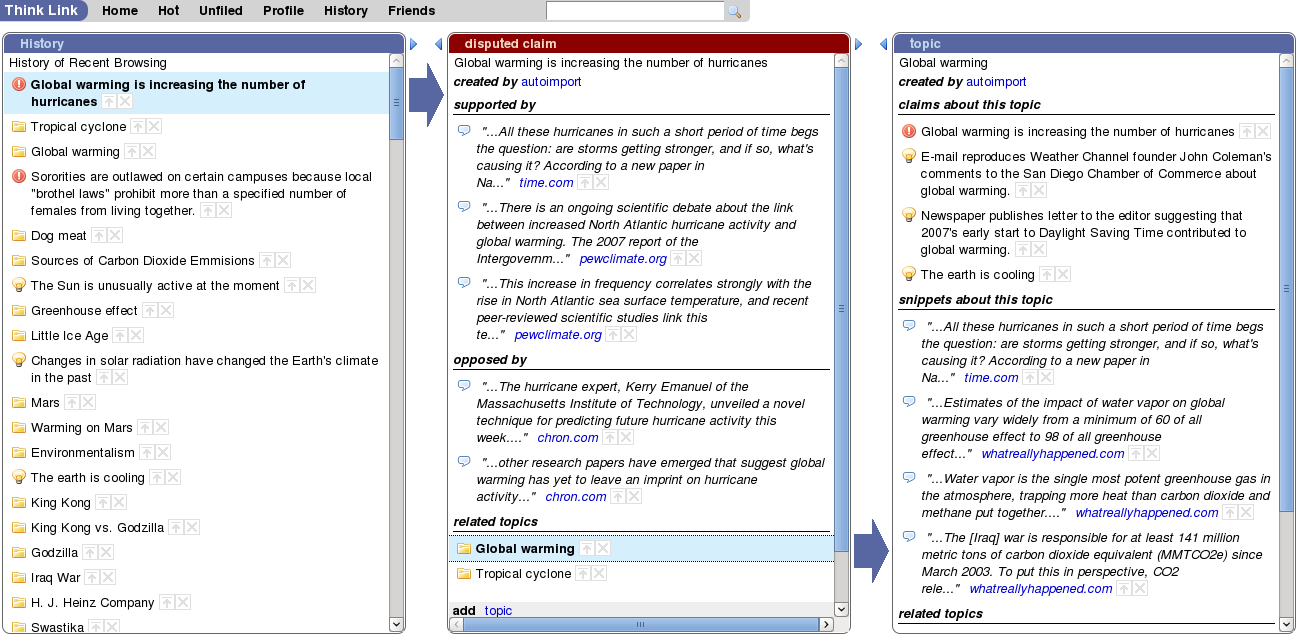
\includegraphics[width=8.5cm]{../screenshots/v2_panels.png}
	\caption{The claim graph consists of a series of linked panels}
	\label{panels}
	\end{center}
\end{figure}

Once a sceptical reader has identified a claim that they are interested in, they can use Think Link's claim browser interface (Figure~\ref{panels}) to investigate the evidence for and against it, and to see what other contentious claims have been made about related issues. 

In our user studies, we found that sceptical readers wanted to be able to investigate the evidence for and against a claim without having to navigate away from that claim. We thus created an interface that consists of a horizontal array of panels where each panel provides information about the item that is selected in the panel to its left. If a panel describes a disputed claim (Figure~\ref{panel}), then a user can investigate a particular piece of supporting evidence by clicking on it and looking at the information in the panel to the right. To emphasis the connection between the panels, the claim browser places an arrow next to each selected item, pointing to the panel that gives more information about that item.

The panel for a claim (Figure~\ref{panel}) lists evidence that will help a user decide whether the claim is true. Evidence is categorized as either supporting, opposing, or being related-to the claim. The ``related-to'' category is used for evidence that does not fit neatly into one side of the argument. Evidence can either be a snippet that talks about that claim, or another claim whose truth would support or oppose this claim. 

\begin{figure}[tb]
	\begin{center}
	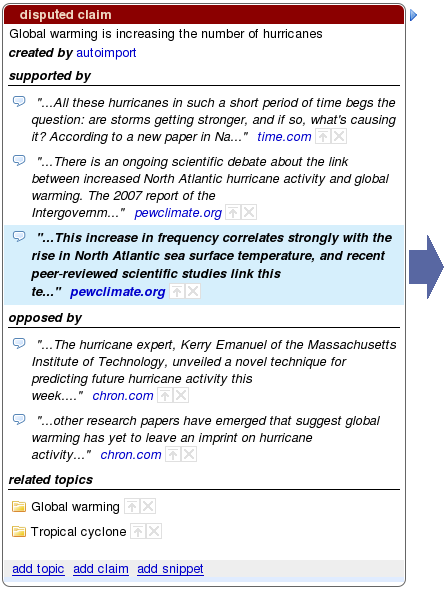
\includegraphics[width=6cm]{../screenshots/v2_panel.png}
	\caption{A claim panel presents information for and against a claim}
	\label{panel}
	\end{center}
\end{figure}

We found that it was important to allow the claim browser interface to be used in two different ways. When a sceptical reader is browsing a web page and sees a disputed claim they want to be able to quickly see a small popup window giving evidence for a disputed claim without having to navigate away from the page~(Figure~\ref{claimview}); however if they are interested in the claim and want to investigate the evidence for a claim in more detail then the small popup interface is too small to easily view large amounts of information and so it is preferable to use a full-window interface. 

To preserve visual consistency, Think Link uses the same claim browser interface for the small popup interface as for the full-window interface. When used as a popup browser, the interface shows only one panel. Clicking on an item in the panel scrolls the display to the right to reveal a new panel in a manner similar to Apple's iPhone. If the user clicks the ``back'' button, the interface will quickly scroll left back to the previous panel.

\begin{figure}[tb]
	\begin{center}
	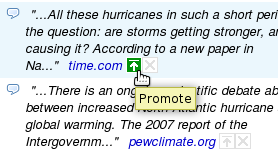
\includegraphics[width=6cm]{../screenshots/v2_vote.png}
	\caption{Voting buttons let users say which evidence is important}
	\label{voting}
	\end{center}
\end{figure}

%\todo{Key issue with hypertext was not talking about things that highlighted arguments?}

Think Link's claim graph is a variant of the IBIS~\cite{Rittel1973} model. There are three types of node: snippets, claims, and topics. A snippet is a region of text taken from a web page; a claim is a statement about the world or position that one can take on some issue; a topic is an issue or concept that a claim might relate to, and a user is a person who users Think Link. Nodes are connected together by typed, directed, links. There are three link types: supports, opposes, and relates-to. A snippet or claim can support, oppose, or relate-to a claim; and any node can relate-to a topic. 

Think Link uses topics to group together related claims. A topic be an issue that several claims are proposing solutions for, for example ``What should we do about global warming?''. Alternatively, it can be a thing that claims are about, for example ``Carbon Dioxide''. Think Link uses the list of page titles on Wikipedia as a seed-set for its topics and users can also add new topics from within the claim browser.

Think Link's graph model is similar to the model used by gIBIS~\cite{Conklin1987} except that we don't distinguish between an argument and a position, we allow a claim to relate-to another claim without supporting or opposing it, we merge issues with topics, we collapse gIBIS's five ways of connecting topics together and four ways of connecting a claim to an topic into a single relates-to relation. The result is a graph structure that is significantly simpler. While Think Link's graph structure is arguably less useful for the argument modelling and resolution task that gIBIS was designed for, it is sufficient for the conflict discovery and snippet organization task that Think Link's graph is intended for, and we have found that the smaller set of link and node types reduces the mential effort required to create an argument graph.

The order in which evidence is displayed is determined by user voting. A user can vote for or against a particular piece of evidence by clicking on the voting button next to that item~(Figure~\ref{voting}). When a user looks at a list of evidence they will see first the things they voted for and then the other evidence ordered based on the number of votes it received from other users.

One danger in a voting system is that a large group of people will drown out the opinions of their opponents by voting down their opinions. Think Link uses several strategies to try to avoid this happening. Firstly, positive votes count for more than negative votes. Thus if two different groups are voting up their own evidence and voting down the opposing group's evidence, it is still likely that the opinions of both groups will be relatively prominent. Secondly, a piece of evidence only competes against other pieces of evidence on the same side of the argument, thus even if supporters of one side are voting up their own evidence, this will not push down evidence on the other side. In some cases, it may still be necessary to introduce a moderation system similar to that used in Wikipedia, where trusted users can override popular opinion when things go wrong.

\todo{Talk about searches}
\todo{Cite work on collaborative filtering}
\todo{Mention the sidebar?}

% If the current page contains snippets then a tab appears in the top left corner of the window. The tab contains a light bulb icon whose color changes according to the nature of the snippets on the page (Figure~\ref{bookmark_icons}) - red if a snippet contains a contentious claim. This allows a user to quickly tell if a page contains something of interest without having to scroll through the whole page. Clicking on the tab opens the margin. The margin provides a summary of all the interesting claims that users have identified on the current page and is designed to mimic the traditional margin notes that readers often write on physical documents~\cite{marginalia}. To emphasize the connection between a margin note and its associated snippet, each margin note is aligned vertically with its snippet and the snippet is highlighted more strongly when the user mouses over the associated margin note. 

\subsection{Campaigning on the Disputed Web}

If a user has installed the Think Link browser extension then they can create a snippet from text on a web page by selecting the text and selecting either ``This is disputed'' or ``This is interesting'' from the context menu. A user selects ``This is disputed'' if they believe that readers of that snippet should be alerted of the fact that a claim that that snippet is making or implying is disputed. A user selects ``This is interesting'' if they believe that the snippet contains useful evidence that could be for readers investigating a disputed claim. 

\begin{figure}[tb]
	\begin{center}
	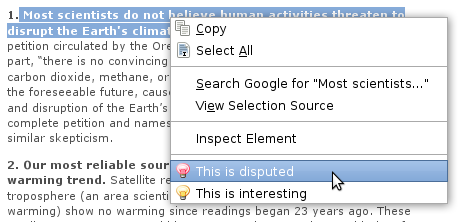
\includegraphics[width=6cm]{../screenshots/v2_snipmark.png}
	\caption{Use the context menu to mark a new snippet}
	\label{createprocess}
	\end{center}
\end{figure}

Think Link does not require that a user associate a snippet with a claim at the point at which they create it. Instead, Think Link encourages a user to associate snippets with claims and topics ``in bulk'' using the claim browser interface, after they have gathered many snippets. One anticipated usage scenario for Think Link is an activist user who uses a search engine to find a large number of snippets that make a clam that they disagrees with. In this case, the user can save time by attaching all the snippets to the same claim together, rather than having to pick the same claim for each one.

Think Link provides three ways for a user to associate a claim with a snippet:

\begin{description}
\item[Claim first:] If a user navigates to a claim and clicks the ``add snippet'' button, Think Link will suggest unattached snippets that the user created recently and that are textually similar to the wording of the claim or other snippets currently attached to the claim (Figure~\ref{snipclaim}). A user can attach a suggested snippet to the claim by clicking on icons representing ``supports'', ``opposes'', or ``relates-to'' link types. If Think Link does not suggest the right snippets then Think Link can guide the suggestions by entering keywords into the text box above the suggestion list.

\begin{figure}[tb]
	\begin{center}
	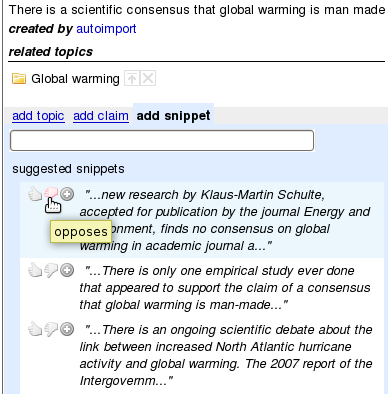
\includegraphics[width=6cm]{../screenshots/v2_sugsnippet.png}
	\caption{Claim first: Pick unfiled snippets to attach to a claim}
	\label{snipclaim}
	\end{center}
\end{figure}

\item[Snippet first:] If a user selects the ``unfiled'' tab at the top of the claim browser then Think Link will show a list of all the snippets that they have marked but not yet associated with a claim or a topic (Figure~\ref{sniptopic}). If the user selects an unfiled snippet then Think Link will suggest claims or topics that the user might want to associate with that snippet. As with the claim-first method, a user can guide the suggestions by entering keywords. If the correct claim is not suggested then the user can create a new claim by typing it into the text box and clicking the ``add'' button.

\begin{figure}[tb]
	\begin{center}
	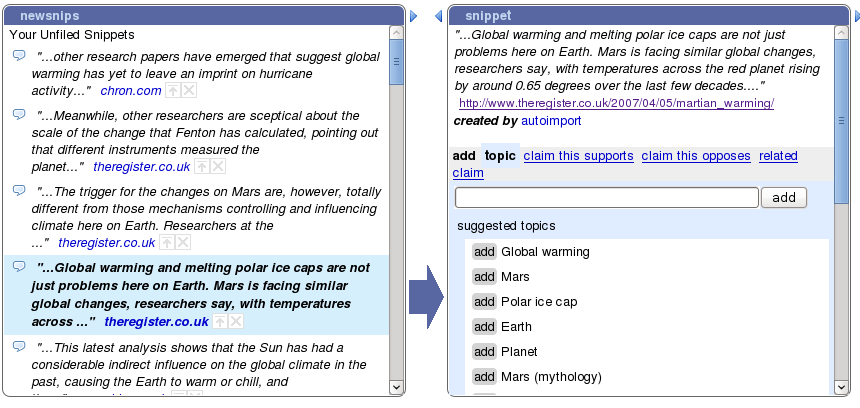
\includegraphics[width=8cm]{../screenshots/v2_sniptopic.png}
	\caption{Snippet first: Pick a claim or topic for each unfiled snippet}
	\label{sniptopic}
	\end{center}
\end{figure}

\item[Immediate:] A user can select a claim for a snippet that they have just marked. When a user marks a snippet, Think Link will initially highlight it in blue to show the user that the snippet is not currently associated with a claim or topic and will not be shown to other users. If the user clicks on the highlighted snippet, then Think Link will bring up the same suggestion panel used in the ``snippet first'' method.
\end{description}

When gathering ``interesting'' snippets, a user may want to associate a snippet with a general topic rather than a specific claim. It is only necessary to associate an ``interesting'' snippet with a claim when a user wants to use it as evidence for a particular claim. In some cases a user will gather snippets that they might want to use later, but without concrete plans for how they might want to use them or what claims they might want to use them as evidence for. In such cases, it is easier to file the interesting snippets under a general topic and possibly attach them to a claim some time in the future. 

As the argument graph grows bigger it becomes increasingly important to make sure that it stays well connected. If different users are interested in the same topic then it is easy for them to create duplicate claims or not connect claims that should be connected. Think Link tries to make it easy for users to keep the claim graph well connected by suggesting claims that should be linked together and allowing a user to connect them with a single click. Think Link uses the same suggestion system to allow users to connect claims to snippets, and to connect claims to other related claims. 

Think Link uses the Wikify algorithm~\cite{Mihalcea2007} to suggest topics for snippets or claims. The Wikify algorithm imagines that a piece of text was on a Wikipedia page and predicts what pages that text would most likely link to based on the probability that any particular n-gram links to any particular page. Recall that the set of Think Link topics is seeded with the set of Wikipedia page titles. The Wikify algorithm performs significantly better than a word-frequency comparison as it biases towards topics that are heavily linked to.

Even with these suggestion and bulk connection features, gathering snippets that make a disputed claim or provide useful evidence requires a non-trivial amount of work. Fortunately, several activist users we talked to told us that they already spend a lot of time performing similar tasks; currently they search for web pages about issues they care about and respond to disputed claims by posting comments or talking about them on their own blog. Some users use tools like Google Alerts\footnote{http://www.google.com/alerts} to be notified every time a new page appears about the issue they are interested in. Moreover, although it would not be practical for activists to mark up all pages on the web, web page popularity follows a Zipf law~\cite{Krashkov2006}, and so one can achive useful coverage by only marking up the relatively small number of very popular pages (for example articles on major news sites).

\todo{Mention about topic previewing}

\todo{Allow two claims to be marked as being identical.}

\todo{BUG: don't have 'add' button for snippets}


\subsection{Implementation}

Think Link consists of a browser extension, a page annotation script, a shared public database of contentious claims, and a web-based argument interface that allows one to explore and manipulate the claim graph. These four components are largely independent of each other and talk to each other using an open API that can also be used by other tools. Indeed the settings panel for the browser extension allows a user to tell it to bind to alternative versions of the other modules.

The page annotation script is a javascript file that can be included into any HTML page. When it is run on a page it sends the page URL to the server, asking it to send back information about any contentious snippets on that page. If any such snippets are found, the page modification script highlights them in red. If the user clicks on a highlighted snippet then it shows an iframe containing a visualization from whatever visualization server it has been configured to use.

The only purpose of the browser extension is to insert the page modification script onto every page that the user loads. The browser extension is not the only way that one can access Think Link highlights. One can get the same effect by browsing through a proxy (like WBI~\cite{Barrett1997}), or if the owner of a web site included the page annotation script themselves.

Think Link's annotation system has some privacy issues. Every time the user browses to a page, the URL is sent to the Think Link server to check whether there are any known annotations for that page. Privacy issues are reduced by the fact that the requests contain no cookies or other identifying information, and can be cached by a third-party proxy if desired; however issues still remain. In future work hope to reduce these privacy issues. One possibility is to use a hashing system similar to that used by Google Safe Browsing\footnote{http://code.google.com/p/google-safe-browsing/}.

The protocol used by the Think Link server is an open REST API that other tools are free to use. We are also considering supporting one or more of the several argumentation interchange formats that have been proposed ~\cite{Rahwan2007a,McGinnis2007}.


\section{User Studies}

We performed two qualitative ``think aloud'' user studies. The aim of these studies was to inform the development of Think Link. The studies were not intended to validate the design of Think Link as being correct. Think Link is designed to be used by a large number of users gathering a vast amount of evidence for many different claims. To confidently state that our design was successful we would need to be able to test Think Link on a much greater scale than we currently have resources for.

The aim of the first study was to see how users normally browse the web and see their reactions to an early version of the Think Link argument graph. The aim of the second study was to evaluate user responses to an updated version of the interface and evaluate how users responded to seeing highlighted snippets on the page. At the end of each study, we asked each partipicant whether there were times in the past where they would have wanted to use Think Link. We present the results of the two studies together.

\todo{Say something about final informal evaluation}
%After the second study, we made minor changes to our user interface (described below) and performed an informal user study with people in our organization to 


\subsection{Procedure for the First Study}

For the first study we recruited 12 paid participants, 5 female, 7 male, aged 18 to 52. Nine participants regularly posted to a blog and the other three regularly posted comments to blogs or mailing lists. Our intention was to recruit users who fit our ``sceptical reader'' and ``activist'' personas. In our advert, we asked people to tell us what kind of information they looked at on the web, and how they shared information with others. We selected participants who looked at information that was likely to be disputed (e.g. political commentry) and said they regularly shared information with friends. We avoided applications from people who were more interested in less disputed topics like social networking or sport.

\todo{Get the correct number of bloggers}

\todo{This was a bad recruiting strategy. We should have recruited people that fitted one of our two personas and then set them tasks that fitted our vision for that persona.}

Study sessions took approximately 45 minutes. Participants were seated at a single-screen workstation with the Firefox browser augmented with the Think Link extension. We first demonstrated Think Link's interface, and then asked them to browse web sites they normally use

the web sites they normally normally and use Think Link to identify snippets that made claims they thought were interesting or disputed and connect those claims to the existing claim graph. For the first half of the study, we asked them to constrain their browsing to political news articles, to increase the likelihood that there would be existing claims about the topic they were browsing.

In this initial study, users were exposed to the prototype interface shown in Figures~\ref{oldsnippetbox} and \ref{oldbrowser}, rather than the final interface described earlier in this paper. We discuss some of the key differences in the findings section.

\subsection{Procedure for the Second Study}

For the second study, we recruited 6 paid participants, 4 female, 2 male. Four participants had a blog. Although we recruited participants using the same advert as the first study, the timing of our second advert around the beginning of the local university semester meant that five of the participants were college students. 

In the second study we were more confident about the usability of our tool and so we decided to tell the participants nothing about how to use it. We gave each user a brief description of the aims of the tool, similar to the introduction of this paper, and then asked them to perform two tasks with it. The first task was to look at a selection of web pages that already had highlighted snippets and explore the interface while thinking aloud about what they saw (the ``sceptical reader'' use case). The second task was to identify disputed claims on a set of pages we gave them about global warming and connect them appropriately to existing claims that we had pre-populated the claim graph with (the ``activist'' use case). 

Participants were shown the prototype interface shown in Figures~\ref{secondbrowser} and \ref{secondsnippetbox}. This was similar to the interface described earlier in this paper, except that it used drag and drop to make connections rather than a suggestion system, it did not offer a ``relates-to'' link between claims, and it required a user to choose a claim at the point at which they create a snippet. 

\subsection{Findings}

In this section we present the findings from our two user studies. Findings from the two studies are presented together and clustered by topic.

\subsubsection{High-Level Impressions}

Response was generally positive, with many participants being very keen to use the tool soon. One participant said ``I can see myself getting addicted to this'', and several participants asked as to notify them when it is properly deployed. Most of the participants expressed an interest in using the tool, with some wanting to use it now, and others wanting to use it ``when it is more mature''.

Most participants said that they would want to use Think Link to tell them when information they read was disputed (sceptical reader). One participant said ``The web needs to be taken with a grain of salt, and this gives you salt goggles''. A smaller number said they would want to marking up claims they disagreed with (activist). One participant who was a political blogger was very excited about the ability to mark up things he thought were lies.

Most participants in the first study, and all participants in the second study were able to use the tool competently. Participants in the second study were able to use Think Link competently without it being demonstrated in advance and were able to correctly deduce what the different parts of the interface meant. One participants said they found the tool ``very intuitive''.

\subsubsection{Choosing a Claim for a Snippet}

\begin{figure}[t]
	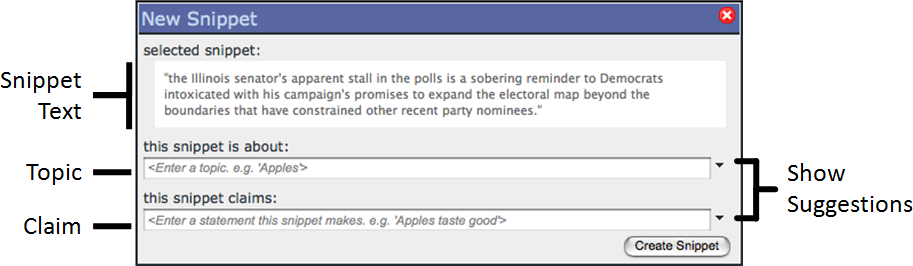
\includegraphics[width=8.5cm]{../screenshots/oldsnipcreate_diagram.png}
	\caption{First Prototype Snippet Creation Dialog}
	\label{oldsnippetbox}
\end{figure}

\begin{figure}[t]
\begin{center}
	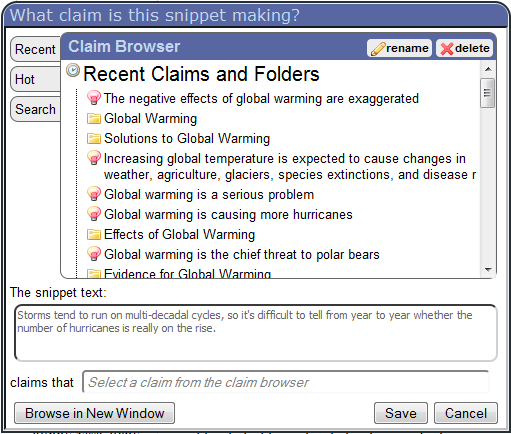
\includegraphics[width=5cm]{../screenshots/newsnip_browseopen.png}
	\caption{Second Prototype Snippet Creation Dialog}
	\label{secondsnippetbox}
\end{center}
\end{figure}

The prototype interfaces required that a user enter a claim for a snippet at the point at which they created the snippet. When the user marked a snippet, Think Link would display a dialog box asking them what claim to associate it with (Figure~\ref{oldsnippetbox} for the first prototype and Figure~\ref{secondsnippetbox} for the second prototype). There turned out to be several problems with requiring that a user select a claim at the point at which they marked a snippet:

Users would often encounter a snippet that could be interpreted as making several interesting claims. Users got confused by the need to pick only one claim. Some users dealt with this by writing a compound claim such as ``Global warming will cause X and Y'', while other users would mark several overlapping snippets making different claims. In the final interface one can associate a snippet with several claims.

Some users wanted to associate a snippet with a topic but without associating it with a specific claim. For example, they might find the text of an important speech, or the results of a sporting event. While it is possible that they might want to use this as evidence for a claim in the future, they didn't want to have to decide what the claim was immediately. In the final interface one can choose to associate a snippet with a topic.

Some users seemed to be deterred from marking interesting snippets by the mental effort required to choose an appropriate claim. In several cases, we saw a user pause to decide whether an interesting snippet was worth marking up. Similarly, some users seemed to find it difficult to decide what the right claim to use for a snippet was, since they had not yet decided how they wanted to structure their argument, or even if this was a topic they wanted to argue about. The final interface does not require a user to associate a snippet with a claim at the time they create the snippet. Instead a user can mark snippets with minimal effort and then later search through their snippets to find evidence for particular claims.

Several users expressed confusion about how specific the claim made by a snippet should be, or when they should pick an existing claim rather than create a new one. For example, if a snippet says ``Global temperatures will rise by X degrees by 2050'' then is that making the claim ``Global temperatures will rise'', or should a new claim be created that contains the extra information? In the final interface, users are expected to only create a claim when they have several snippets that make the same claim. This makes it easier to know how broad the claim should be as they know how much information is shared by claims.

Since a user was required to enter a claim whenever they created a snippet, there was an incentive for the user to enter a claim as quickly as possible so they they could make the dialog go away. Several users created a new claim that was equivalent to a claim that already existed, and several users repeatedly created a claim that had the exact same text as the snippet. The final interface reduces this problem by not requiring a user to associate a claim with a snippet until they decide that this is something that they want to do, and have a particular disputed claim in mind.

\todo{Need to do some kind of evaluation to show that the new interface solves these problems}


\subsubsection{Choosing what to mark as a snippet}

Many users would consistently mark the first paragraph of an article as a snippet. This paragraph would frequently summarize the arguments made in the rest of the document document and often made an important claim that other claims in the document supported or provided context for. 

Several users wanted to mark up a table or an image as a snippet. This is valid behavior -- a table or image is often useful evidence for a claim; however it is not currently supported by Think Link. In future versions of Think Link we intend to support this behavior.


\subsubsection{Connecting Claims}

Many participants expressed a desire to organize claims into connected arguments during their session. 

Some users marked one claim as supporting another when it would have been more logically correct to make them both as supporting a third claim that needed to be created. For example ``Global warming is causing more hurricanes'' does not support ``Global warming is causing rising sea levels'', but both support ``Global warming is causing problems''. Users realized that the claims were related, but were not sure how best to connect them. It is possible that creating logically correct claim structures may be too difficult for some people (see Isenmann and Reuter~\cite{Isenmann1997}). We believe that this problem can be addressed to some extend though voting by other users who recognize that a claim does not provide useful evidence.

Some users were confused by claims that had a ``because'' relationship rather than a ``supports'' or ``opposes'' relationship. For example ``America did not sign the Kyoto Protocol'' {\it because} ``Signing Kyoto would harm the US economy''. Similarly, many users expressed a desire to mark claims as being related without supporting or opposing each other. For example ``America did not sign the Kyoto Protocol'' {\it  relates-to} ``America was right to not sign the Kyoto Protocol''. In the final interface we introduced a ``relates-to'' link type to allow users to connect claims that they thought should be related but which didn't confirm to a simple pro/con relationship. 

Several users got confused by claims that referred to similar events at different points in time. For example, one participant in the first study marked a two claims as opposing each other when each was true at the time that it was written. This is a particular problem when talking about breaking news events, where what claims are true can change fast. If Think Link is to be effective for describing such events then it is likely that it will need to have better support for identifying the time at which a claim was asserted to be true.

Several users expressed an interest in being able to mark a claim as controversial without having to create an opposing claim. One user said that opposing a claim required ``too many clicks'' and they wanted to be able to just vote against a claim without having to say why or find evidence. In the future we are planning to implement a social voting system to allow users to say what claims they believe are false and see what claims their friends agreed or disagreed with.

\begin{figure}[tb]
	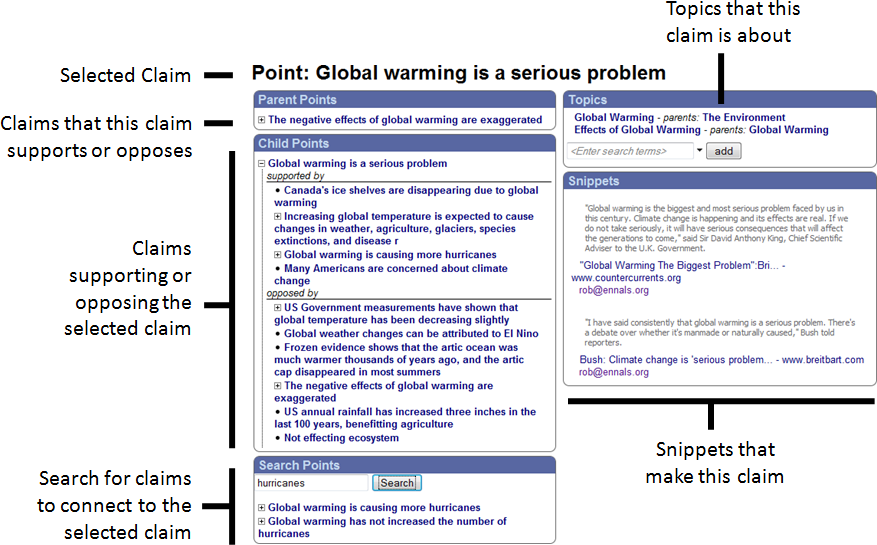
\includegraphics[width=8.5cm]{../screenshots/oldpoint_diagram.png}
	\caption{First Prototype Claim Browser}
	\label{oldbrowser}
\end{figure}

\begin{figure}[tb]
\begin{center}
	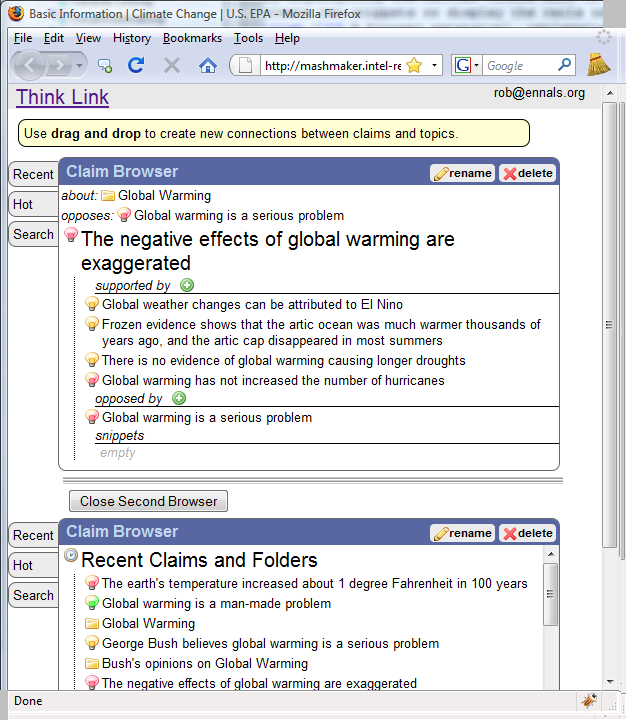
\includegraphics[width=5cm]{../screenshots/claimbrowse.png}
	\caption{Second Prototype Claim Browser}
	\label{secondbrowser}
\end{center}
\end{figure}

The first two versions of Think Link used a drag-and-drop interface to allow a user to create links between claims. In the first interface (Figure~\ref{oldbrowser}) a user could use a search box to find other claims and then drag them into an appropriate position in the argument tree. In the second interface (Figure~\ref{secondbrowser}), followed a file-manager metaphor, providing two identical browser windows that a user could drag and drop claims between. In both cases, we found that users would often not intially realize they could use drag and drop to organize claims, even when we added a prominent information message at the top of the display (Figure~\ref{secondbrowser}). We believe that part of the problem was that users are not used to using drag-and-drop in a web interface, and there was no visible clue in the rendering of the claim graph that they could use drag and drop to create connections. In the final interface we resolved this issue by having the connection actions (``add claim'' etc) explicitly visible in the interface.

\section{Future Work}

At present Think Link relies on users to mark up snippets and connect them to claims. In the future we plan to explore using natural language and machine learning techniques to assist in this process. Our plan is to allow a user to request that Think Link present them with potential web snippets that make a claim that they disagree with, and then quickly select which of these should be highlighted as being contentious.

Think Link is designed to be used as a social tool in which large numbers of people collaborate to find large numbers of claims and snippets about interesting topics. Since our graph and user base are currently small, we have not yet evaluated how Think Link works when data sets are huge, many users are concurrently editing data, and some users are malicious.

We think it could be useful to use Think Link as a tool to suggest reading material. Just as tools like Digg suggest pages that you might like, Think Link could potentially suggest pages that contain claims that the user had not read and would be likely to find interesting.

\section{Conclusions}

We have introduced the idea of enhancing the browsing interface by highlighting snippets of text that make disputed claims and allowing a user to see an argument graph that presents the best evidence on either side of the issue. Think Link allows users to navigate between pages based on the factual claims made on pages, rather than being restricted to the links provided by authors. It allows users to identify disputed claims on web pages and connect them directly to the arguments that those claims are part of, and related claims on other web sites.

On a practical level, Think Link works by allowing users to pick out snippets on pages that make claims that they think are interesting or controversial, and then using a collaborative filtering model to allow users to vote for the most interesting evidence and structure claims into a coherent argument graph.

We hope that Think Link will make it easier for people to be informed about the world and be exposed to factual claims that they might not otherwise be exposed to.

\section{Acknowledgments}

Acknowledgements omitted for blind submission. Think Link uses icons from the free FamFamFam Silk\footnote{http:\\famfamfam.com} collection.


\todo{Sort out bad references}
\bibliography{refs}

\end{document}



